\subsection{Fragebogen} \label{fragebogen-1}

\todo[inline,color=green!40]{Verantwortlich: Boris\\
- RfP}

Ein Fragebogen kann als Formular definiert werden, das einen Satz von Fragen enth{\"a}lt, die f{\"u}r einen bestimmten Zweck definiert wurden\cite{gault-questionnaire}.
Hier dient der Fragebogen als Befragungsinstrument f{\"u}r die Realisierung unseres Projekts. 
Hierf{\"u}r wurden f{\"u}­r die Ausarbeitung die Hauptkomponenten definiert, die Auskunft {\"u}ber das Problem der Studie und {\"u}ber die Versuchsperson geben. \\

F{\"u}r das erste Experiment dieser Studie sieht das Fragebogenmodell folgendes aus: eine Liste von elf Emotionen (Angst, Aufregung, Frustration, Langeweile, Neugier, Ruhe, Traurigkeit, {\"u}berraschung, Wut, Befriedigung und Nervosit{\"a}t) mit je vier nummerierten  Check-Boxen, die nach der Intensit{\"a}t des Gef{\"u}hls der betreffenden Emotion angekreuzt werden sollten. 
Das erste Feld entspricht der niedrigsten Intensit{\"a}t und das vierte Feld der h{\"o}chsten Intensit{\"a}t. Man hat auch die M{\"o}glichkeit, keine Check-Box auf eine Emotion anzukreuzen, wenn man seiner Meinung nach die Emotion gar nicht gesp{\"u}rt hat. 
Das w{\"u}rde dem Intensit{\"a}t Null entsprechen. 
Zudem soll man auch f{\"u}r jedes Viertel der Zeit eines Szenario die dominante Emotion w{\"a}hlen. \\


\begin{figure}[H] \centering
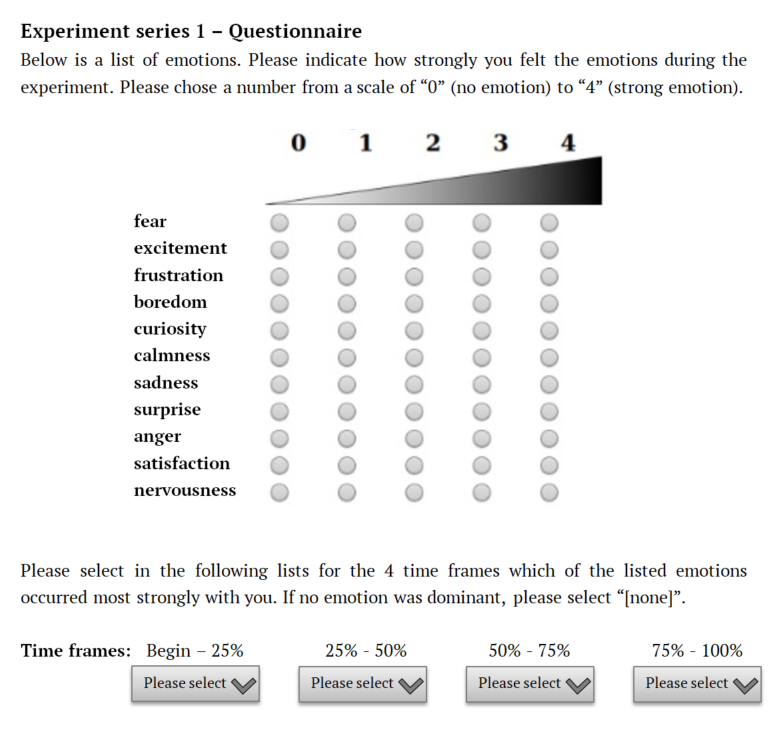
\includegraphics[width=\textwidth]{Images/questionnaire-1.png} 
\vspace{-0.3cm} 
\caption{Bild des verwendeten Fragebogens.}
\label{fig-questionare-1} 
\end{figure}

